\section{Results}
\label{sec:results}
\paragraph{Performance metrics}
\Cref{tab:scores-dialog} and \Cref{tab:scores-narration} show
the performance of several model configurations on the retrieval and
triplet tasks on the dialog and narration datasets respectively.

In the case of the narration data this scores is not confounded by
speaker-based clues, which is an indication that the model possibly
learned to detect some aspects of utterance meaning. We investigate
this hypothesis further using multiple representational similarity
analysis.
 

 \begin{table}
   \centering
   \begin{tabular}{rlrr}
\toprule
 ID & Pretraining &  Recall@10 &  Triplet Acc \\
\midrule
 43 &          AV &      0.193 &        0.814 \\
 44 &           V &      0.084 &        0.728 \\
 45 &        None &      0.034 &        0.597 \\
\bottomrule
\end{tabular}

   \caption{Retrieval and triplet scores on dialog validation data.}
   \label{tab:scores-dialog}
 \end{table}

\begin{table}
   \centering
   \begin{tabular}{rlrr}
\toprule
 ID & Pretraining &  Recall@10 &  Triplet Acc \\
\midrule
 43 &          AV &      0.239 &        0.866 \\
 44 &           V &      0.166 &        0.822 \\
 45 &        None &      0.087 &        0.741 \\
\bottomrule
\end{tabular}

   \caption{Retrieval and triplet scores on narration validation data.}
   \label{tab:scores-narration}
 \end{table}
 
\paragraph{Targeted Triplets}
\todo{add average targeted triplets result to general performance metrics table?}

The best performing model according to the
performance metrics (ID 48, audio and video pretraining) achieves an average
targeted triplets accuracy of 0.719 . \Cref{fig:accuracy_targeted_triplets_nouns} and
\Cref{fig:accuracy_targeted_triplets_verbs} show per-word
accuracy for nouns and verbs, respectively. The vertical
bars indicate the standard deviation as estimated using bootstrapping
tests.

We further compute correlations between the per-word accuracy and two possible predictors of age of acquisition: frequency and concreteness. The resulting correlations are presented in Appendix \ref{app:targeted_triplets_eval}. There is a significant positive correlation between word concreteness and the model's accuracy for this word. Regarding input frequency, we find no significant correlation.

As a baseline, we evaluate the same model (pretrained) without being fine-tuned on our dataset. The resulting performance is as expected close to chance level: 0.538 .


\begin{figure}
  \centering
  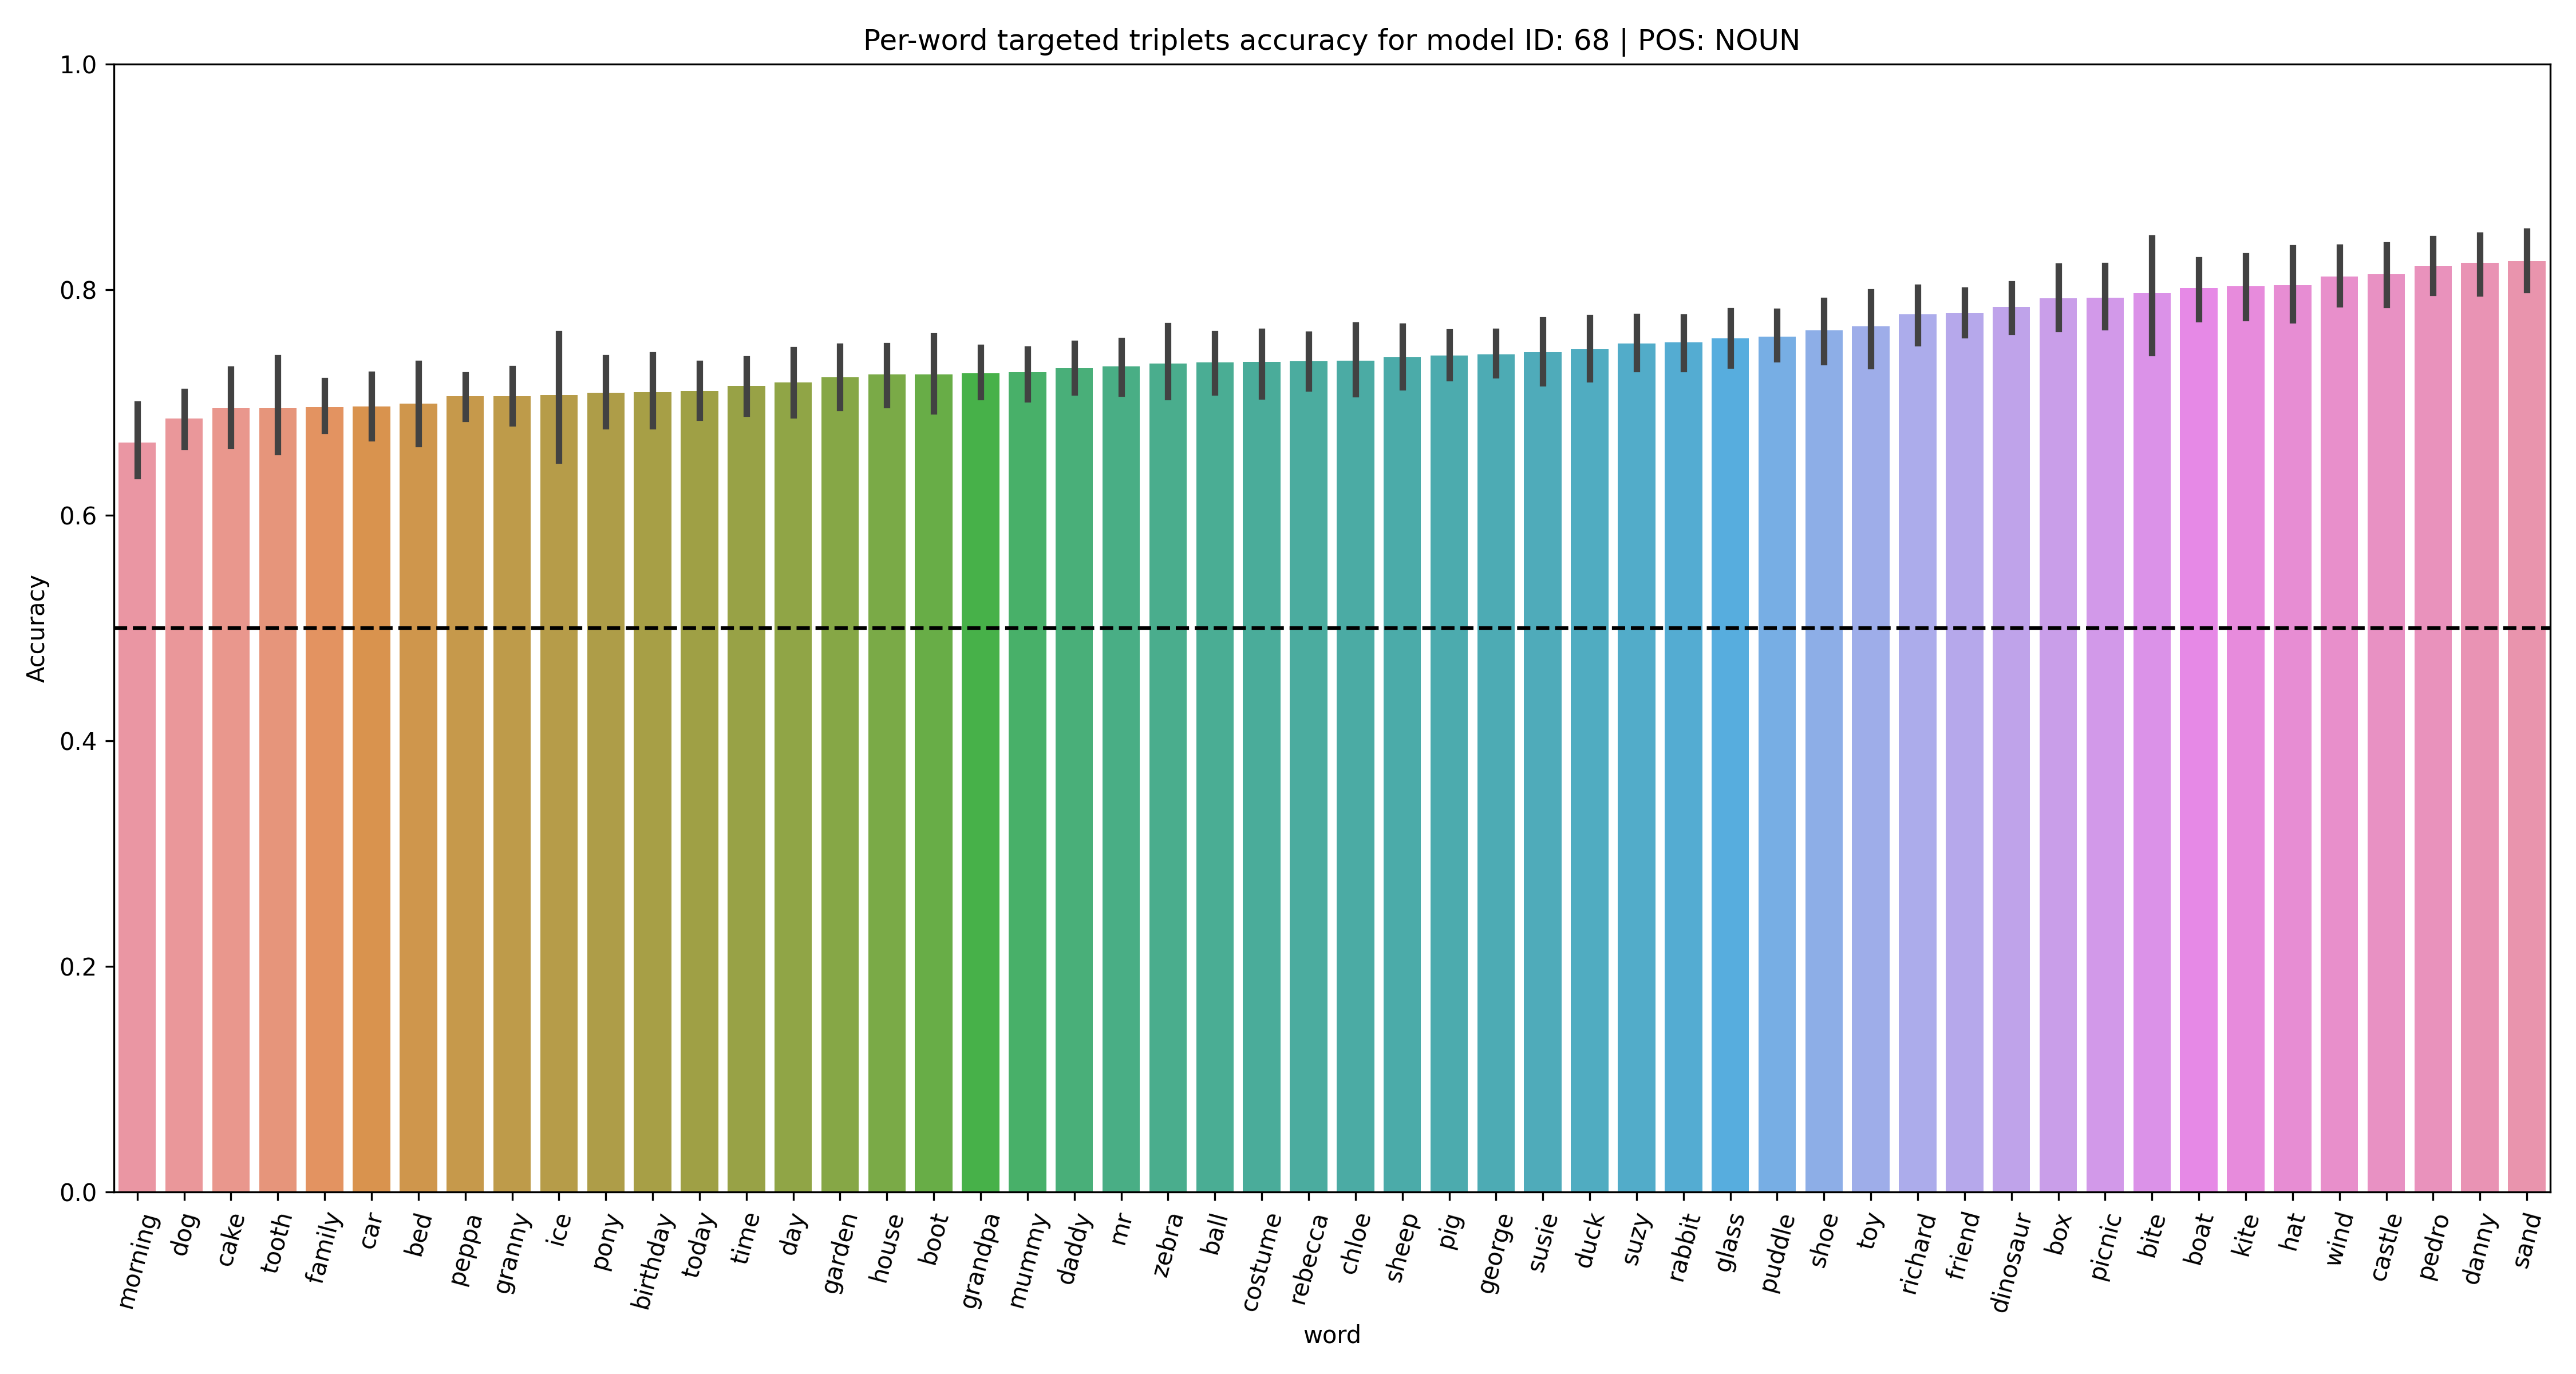
\includegraphics[width=\textwidth]{results/targeted_triplets/results_NOUN_word.png}
  \caption{Per-word targeted triplets accuracy for nouns.}
  \label{fig:accuracy_targeted_triplets_nouns}
\end{figure}

\begin{figure}
  \centering
  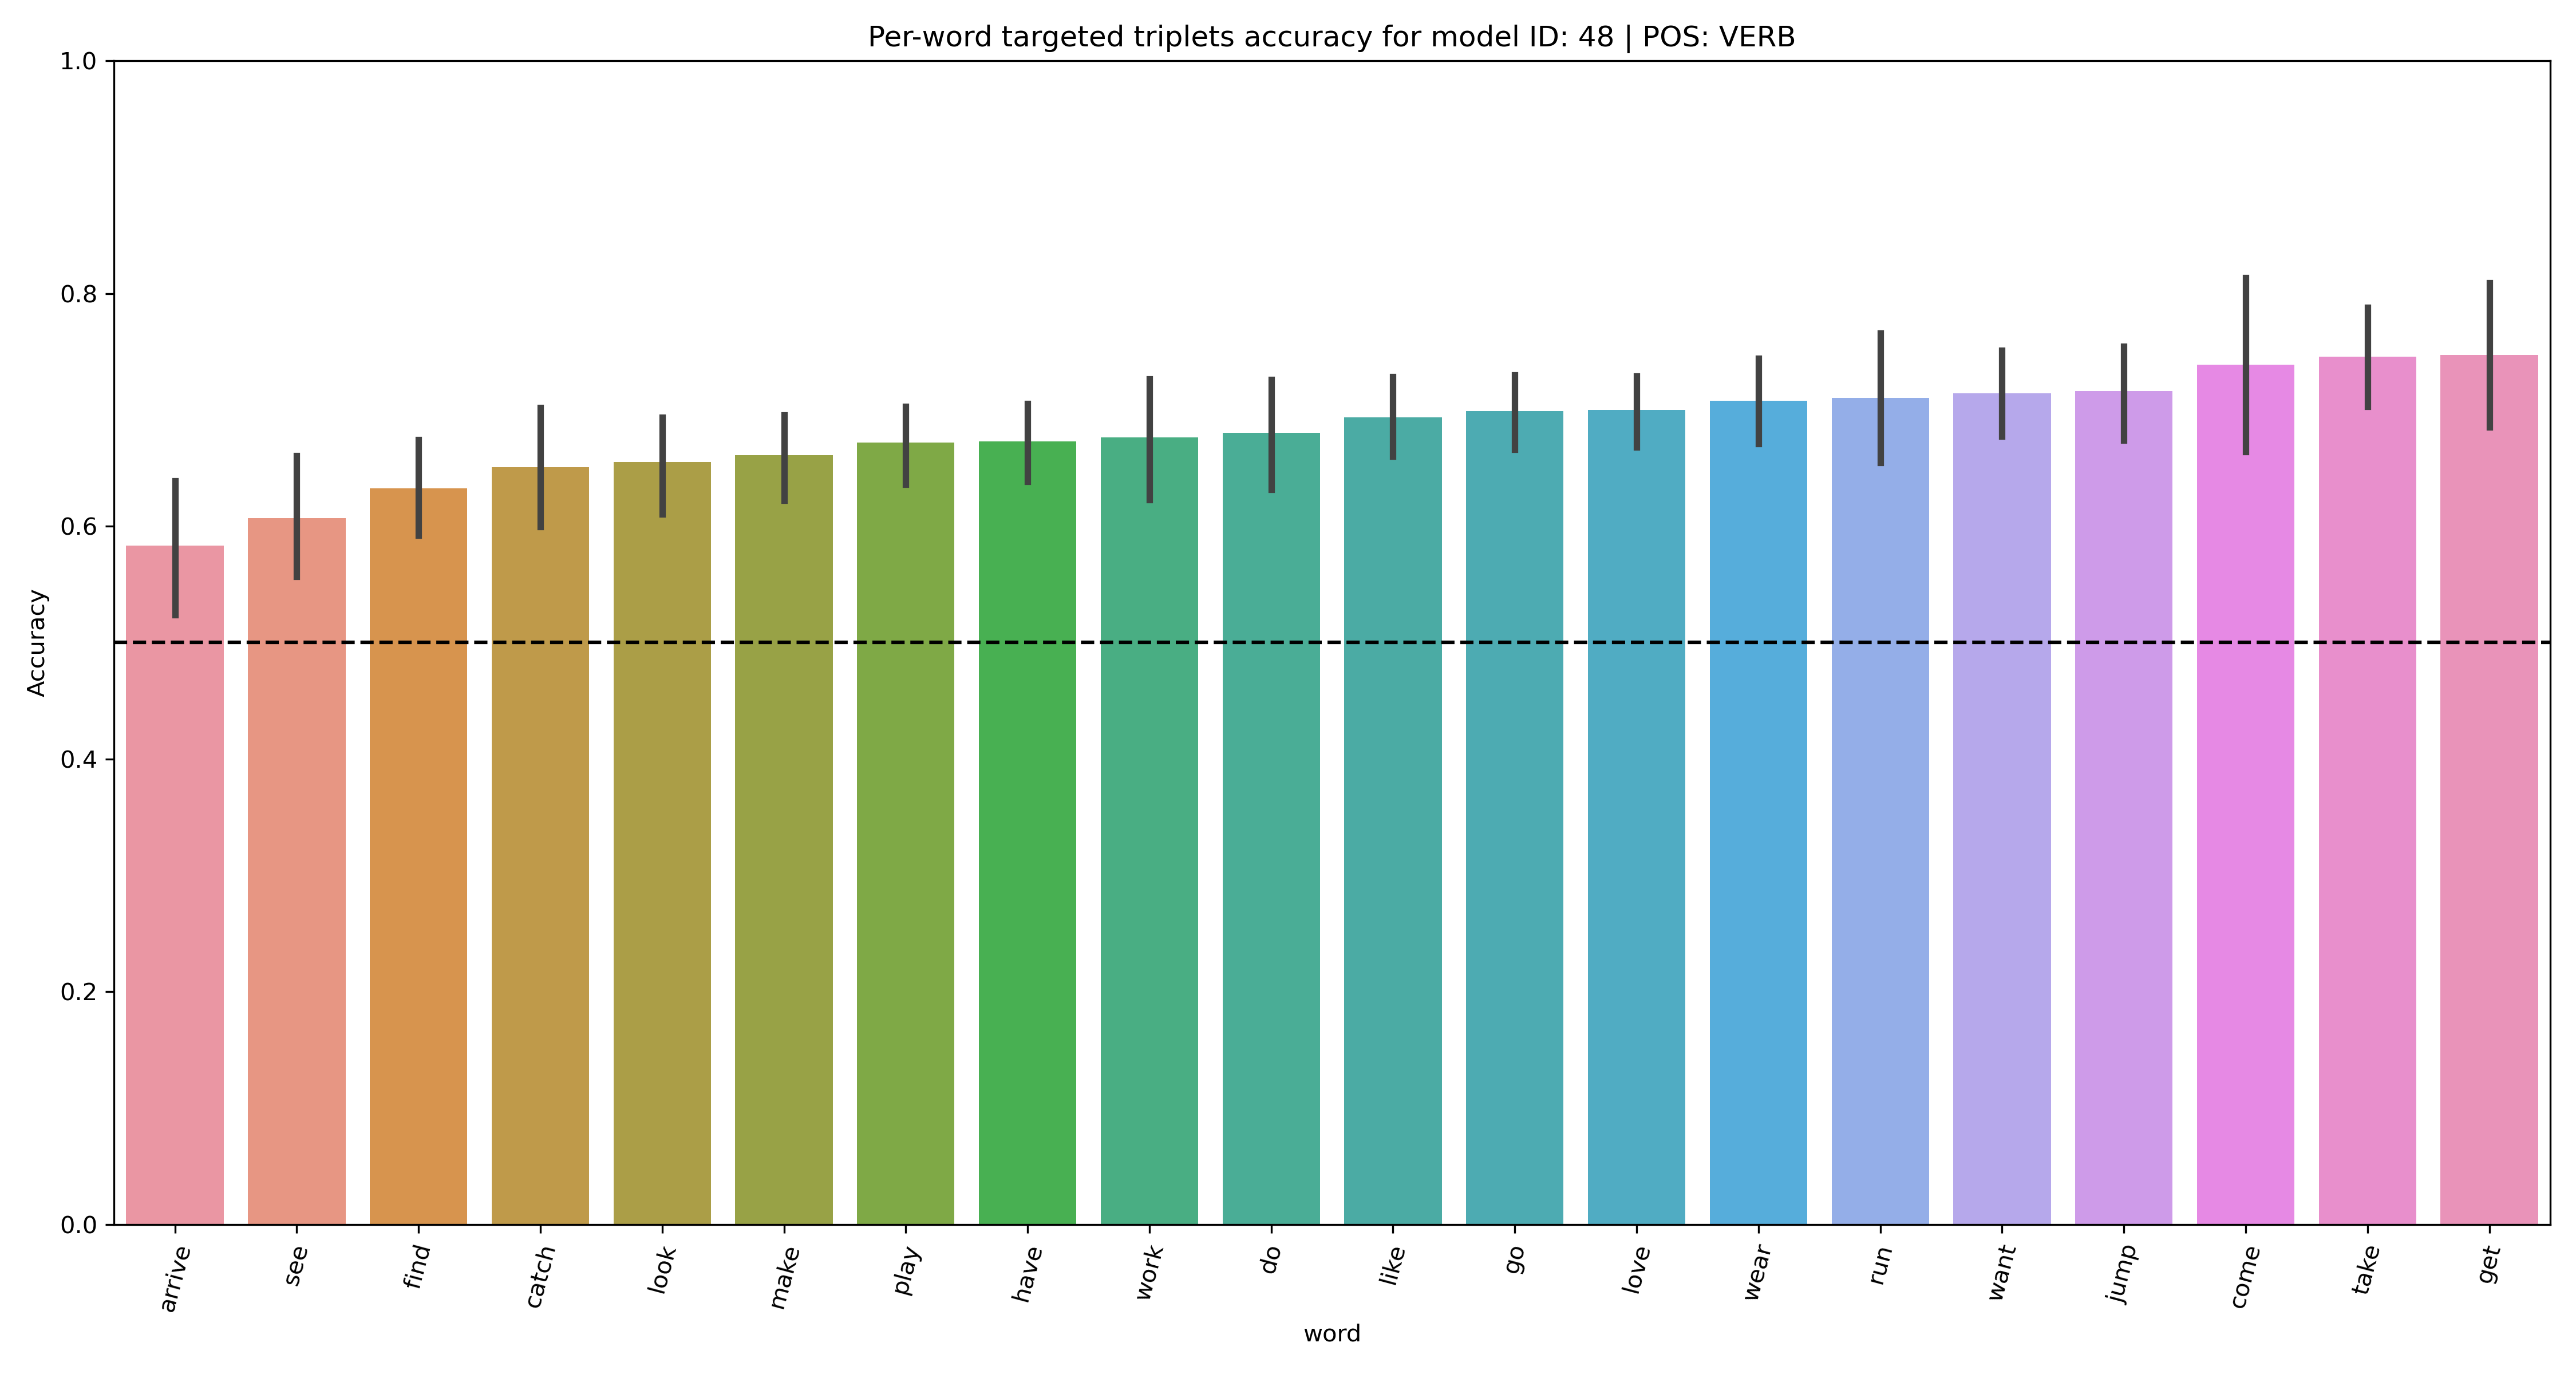
\includegraphics[width=\textwidth]{results/targeted_triplets/results_VERB_word.png}
  \caption{Per-word targeted triplets accuracy for verbs.}
  \label{fig:accuracy_targeted_triplets_verbs}
\end{figure}

 
